%===========================================================
%
% Dedman/Lyle LaTeX Dissertation Template, v.2016
% Structure organized by Ted C. Munger (TCM)
%
%===========================================================
%===========================================================
% BEGIN Document Style
%===========================================================
\documentclass[12pt, draft]{report}

%\makeatletter
%\DeclareOldFontCommand{\rm}{\normalfont\rmfamily}{\mathrm}
%\DeclareOldFontCommand{\sf}{\normalfont\sffamily}{\mathsf}
%\DeclareOldFontCommand{\tt}{\normalfont\ttfamily}{\mathtt}
%\DeclareOldFontCommand{\bf}{\normalfont\bfseries}{\mathbf}
%\DeclareOldFontCommand{\it}{\normalfont\itshape}{\mathit}
%\DeclareOldFontCommand{\sl}{\normalfont\slshape}{\@nomath\sl}
%\DeclareOldFontCommand{\sc}{\normalfont\scshape}{\@nomath\sc}
%\makeatother


  \usepackage{DL_thesis_v2016}  % TCM Global Style for particular SMU College, e.g. DL_thesis_v2016.sty

  %--------------------------------------------------------------------------------------------------------
% 									LaTeX Package File
%
% TCM Use this file to add, modify, or comment out packages you want to utilize in your Latex project.
%     This file must be included in the main document file.
%--------------------------------------------------------------------------------------------------------

\usepackage{adjustbox}       % TCM Extends the graphicx package to do trimming and other adjustments.
\usepackage{algorithm}       % TCM Algorithm block See http://algorithms.berlios.de/
\usepackage{algorithmic}     % TCM Algorithm & Peudocode See http://en.wikibooks.org/wiki/LaTeX/Algorithms_and_Pseudocode
\usepackage{amsmath}         % Need for subequations
%\usepackage{amssymb}        % amssymb-telda and math symbols
\usepackage{booktabs}        % TCM Allows fancy Tables
\usepackage{boxedminipage}   % Boxes around figures
\usepackage{breqn}           % TCM Automatically breaks long equation lines - usually
\usepackage{changepage} 	 % TCM Allows one to temporarily change right and left margins
\usepackage{cite} 	 		 % TCM Allows improved handling of numeric citations including automatic ordering and ranges of multiple cites
\usepackage{enumitem} 		 % TCM Allows one to easily change the labels for enumerate list
%\usepackage{epsf}           % TCM This EPS file package is greatly depreciated for the graphicx package bundle. Use at own risk.
\usepackage{fancyhdr}
\usepackage{flafter}         % Floats should always appear after their definition
\usepackage[flushleft]{threeparttable}  % TCM This package allows for notes under tables.  Flushleft option flushes the note left margin of table (center is default)
\usepackage{geometry}		 % TCM Allows to customize paper size and margins.
\usepackage{graphicx}        % TCM Extends graphics package for figures. Provides op­tional ar­gu­ments to the \in­clude­graph­ics com­mand
\usepackage{epstopdf}        % TCM Converts eps images to PDF to use in graphicx package.  Must be loaded after graphicx package
\usepackage{longtable}       % TCM Allows for Automatic page breaks for long tables
%\usepackage{jneurosci}       % TCM The jneurosci bibliography style makes use of some commands - for example, \citeauthoryear.  Must include if using named or acmsmall bib style
\usepackage{ltablex}		 % TCM Modifies Tabularx Package by combining properties of tabularx and longtable.
\usepackage[maxfloats=36]{morefloats}      % Latex will handle more floats 18-36
\usepackage{moresize}        % TCM Adds \HUGE and \ssmall font sizes
\usepackage{multirow}        % TCM Allows multirow cells in tables (similar to merge and center in Excel)
%\usepackage{named}           % TCM Bibliography style that allows for more fine-tuned citing. Commands include \cite, \citeauthor, \citeyear and \shortcite (for after you've already used \citeauthor).
\usepackage{outlines}		 % TCM Needed for outlines
\usepackage{rotate}			 % TCM Performs rotations of floating environments (images w/ cations, etc)
\usepackage{rotating}        % Need for sidewaystable
\usepackage{scrextend}		 % TCM package that allows for KOMA-Script classes available for other classes: e.g., labeling lists etc.  See package documentation for further information.
\usepackage{pdflscape}		 % TCM Allows Landscape Page
%%\usepackage{qtree}         % Need for trees
\usepackage{setspace}        % TCM Allows for more intuitive commands for single and double spacing
\usepackage{siunitx}		 % TCM package required to ensure units are typeset properly with numbers e.g. \SI{10}{\kg\m\per\square\s}
\sisetup{output-exponent-marker=\ensuremath{\mathrm{E}}}  % TCM Option allows for Scientific notation of Numbers.  Format is \num{#.####E##}
% \usepackage[superscript]{cite}		  % TCM Makes citations superscript instead of [#]
\usepackage [table]{xcolor}	 % TCM Allows coloring of tables
\usepackage{tabularx}		 % TCM Package which allows paragraphs in Tables
% \usepackage{thumbpdf}		  % TCM Comment out as causes warnings, can easily create thumbs in Adobe if needed.

%===========================================================
% BEGIN Color ToDo Comment Notes for editing
%===========================================================
\usepackage[colorinlistoftodos,textwidth=25mm,shadow,backgroundcolor=green]{todonotes}				  % TCM Allows margin comments
\usepackage{marginnote}				  % TCM Require for Todonotes in Align Envionment
  %~~~~~~~~~~~~~~~~~~~~~~~~~~~~~~~~~~~~~~~~~~~~~~~~~~~~~~~~~~~
  % TCM  BEGIN Altering Todonotes Commands to use Marginnote instead of Marginpar to use todonotes in align environment
%~~~~~~~~~~~~~~~~~~~~~~~~~~~~~~~~~~~~~~~~~~~~~~~~~~~~~~~~~~~
     \makeatletter
     \renewcommand{\@todonotes@drawMarginNoteWithLine}{%
     \begin{tikzpicture}[remember picture, overlay, baseline=-0.75ex]%
         \node [coordinate] (inText) {};%
     \end{tikzpicture}%
     \marginnote[{% Draw note in left margin
         \@todonotes@drawMarginNote%
      \@todonotes@drawLineToLeftMargin%
     }]{% Draw note in right margin
         \@todonotes@drawMarginNote%
         \@todonotes@drawLineToRightMargin%
     }%
     }
     \makeatother
       %----------------------------------------------------
       % TCM  BEGIN New Todonotes Command to use single line spacing (sls) in note
       %----------------------------------------------------
       \newcommand{\slstodo}[2][]
       {\todo[caption={#2}, size=\small, #1]{\renewcommand{\baselinestretch}{0.5}\selectfont#2\par}}
       %----------------------------------------------------
       % TCM  END New Todonotes Command to use single spacing in note
       %----------------------------------------------------
       
  %~~~~~~~~~~~~~~~~~~~~~~~~~~~~~~~~~~~~~~~~~~~~~~~~~~~~~~~~~~~
  % TCM  END Altering Todonotes Commands to use Marginnote instead of Marginpar to use todonotes in align 
%~~~~~~~~~~~~~~~~~~~~~~~~~~~~~~~~~~~~~~~~~~~~~~~~~~~~~~~~~~~
%===========================================================
% END Color ToDo Comment Notes for editing
%===========================================================

\usepackage{verbatim}        % TCM Verbatim text block
\usepackage{wrapfig}         % Wrap figures
\usepackage{xspace}          % Allows dynamic space in global text variables. This can allow you to just use \newCommandName rather than \newCommandName{}.
\usepackage [bookmarks=true,backref=page, hyperfigures=true, pdfpagelabels=false] {hyperref}
%===========================================================
% BEGIN Hyperlink Setup
%===========================================================
\hypersetup{
									  % TCM Added more precise definition and options for Hyperref package.
									  % TCM Comment out or change hyperref preferences
									  % TCM \hypersetup should be loaded last 
    bookmarksopen=true,				  % True: Open bookmark tree
    bookmarksnumbered=true, 		  % True: put section numbers in bookmarks
    breaklinks=true,				  % True: split the url over multiple lines
%    draft=true,						  % True: do not do any hyper linking
    filecolor=magenta, 				  % Color of file links
    citecolor=blue, 				  % Color of links to bibliography
    colorlinks=true, 				  % False: boxed links; true: colored links
    linkcolor=blue, 				  % Color of internal links
    linktocpage=true, 				  % True: Makes the page number of TOC the link vs the text
%    pagebackref=true,				  % True: Links references back to referring page
    pdfnewwindow=true,         		  % True: URL links in new window
    plainpages=false, 				  % True: do page number anchors as plain Arabic
    pdffitwindow=false,        		  % Window fit to page when opened
    pdfmenubar=true,           		  % Show Acrobat menu
    pdfstartview={FitH},       		  % Fits the width of the page to the window
    pdftoolbar=true, 				  % Show Acrobat toolbar
    pdfauthor={Author}, 			  % Author in PDF document properties
    pdfcreator={Author}, 			  % Creator of the document in PDF document properties
    pdfkeywords={Keyword1} {Keyword2} {Keyword3} {Keyword4} {Author}, % List of keywords in PDF document properties
    pdfproducer={Producer}, 		  % Producer of the document in PDF document properties
    pdfsubject={Subject},   % Subject of the document in PDF document properties
    pdftitle={Title of Dissertation}, % Title in PDF document properties
    unicode=false,             		  % Non-Latin characters in Acrobat bookmarks
    urlcolor=cyan 					  % Color of external links
}
%===========================================================
% END Hyperlink Setup
%===========================================================
\usepackage{bookmark}		 		  % TCM Eliminates Warning Bookmark level greater than one.  Must be loaded after Hyperref

%===========================================================
% Arya's Packages
%===========================================================
\usepackage{tgpagella}		 		  % ADM Let's use Papyrus. It really classes up this whole affair.
\usepackage{microtype}		 		  % ADM While we're at it, so does improved kerning.
% \usepackage[font=small,labelfont=bf,hypcap]{caption}
%\usepackage{mathtools, amsmath, amsfonts, amssymb}
\usepackage{dirtytalk}
\usepackage{bm}  % ADM Bold math symbols
               % Packages File

  \geometry{letterpaper, margin=1in} % TCM Dedman/Lyle Standard 2016


  \linespread{1.6}
  \setcounter{secnumdepth}{4} % TCM Sets number subsections
  \setcounter{tocdepth}{4}    % TCM Set the number of subsections in TOC
  
   \urlstyle{same} % TCM Set URL style to same font as text verses mono-spaced, i.e., courier

%===========================================================
% END Document Style
%===========================================================
%===========================================================
% BEGIN Insert Custom Commands
%===========================================================
  %======================================================================
% Custom Commands  Inital Creation TCM 2015
%======================================================================
% Use this document to place all of your global new commands
%======================================================================

%======================================================================
% BEGIN SMU Custom Commands
%======================================================================
% The many of the following commands were originally in the smu_thesis.sty
% file. Commands and comments were moved here to make style file more about
% document style. While custom environments can technically be considered 
% style, the student created environments are included here to simplify
% the style file. Often these commands were created by students over the
% years and placed in the style file.  The commands have not been 
% verified and can be obsolete LaTeX commands. The Commands can be used 
% or ignored. 
%======================================================================
%----------------------------------------------------------------------
% BEGIN TCM Commands to set formatting for Paragraph section to have line
%           feed after heading & Numbered. This custom command makes
%           \paragraph, in essence, a form of \subsubsubsection.
%           Uncomment to use.
%----------------------------------------------------------------------
%  \makeatletter
%  \renewcommand\paragraph{\@startsection{paragraph}{4}{\z@}%
%    {-3.25ex\@plus -1ex \@minus -.2ex}%
%    {1.5ex \@plus .2ex}%
%    {\normalfont\normalsize\bfseries}}
%  \makeatother
%----------------------------------------------------------------------
% END of Commands to set formatting for Paragraph section to have line
%       feed after heading TCM
%----------------------------------------------------------------------
%----------------------------------------------------------------------
% BEGIN Shortcuts to insert calligraphic letters in Math Mode Only
%----------------------------------------------------------------------
\newcommand{\cA}{{\mathcal A}}
\newcommand{\cB}{{\mathcal B}}
\newcommand{\cC}{{\mathcal C}}
\newcommand{\cD}{{\mathcal D}}
\newcommand{\cE}{{\mathcal E}}
\newcommand{\cF}{{\mathcal F}}
\newcommand{\cG}{{\mathcal G}}
\newcommand{\cH}{{\mathcal H}}
\newcommand{\cI}{{\mathcal I}}
\newcommand{\cJ}{{\mathcal J}}
\newcommand{\cK}{{\mathcal K}}
\newcommand{\cL}{{\mathcal L}}
\newcommand{\cM}{{\mathcal M}}
\newcommand{\cN}{{\mathcal N}}
\newcommand{\cO}{{\mathcal O}}
\newcommand{\cP}{{\mathcal P}}
\newcommand{\cQ}{{\mathcal Q}}
\newcommand{\cR}{{\mathcal R}}
\newcommand{\cS}{{\mathcal S}}
\newcommand{\cT}{{\mathcal T}}
\newcommand{\cU}{{\mathcal U}}
\newcommand{\cV}{{\mathcal V}}
\newcommand{\cW}{{\mathcal W}}
\newcommand{\cX}{{\mathcal X}}
\newcommand{\cY}{{\mathcal Y}}
\newcommand{\cZ}{{\mathcal Z}}
% Lower case caligraphy letters
\newcommand{\cw}{{\mathcal w}}
%----------------------------------------------------------------------
% END Shortcuts to insert calligraphic letters in Math Mode Only
%----------------------------------------------------------------------
%----------------------------------------------------------------------
% BEGIN Shortcuts to insert boldface letters 
%----------------------------------------------------------------------
\newcommand{\bA}{{\bf A}}
\newcommand{\bB}{{\bf B}}
\newcommand{\bC}{{\bf C}}
\newcommand{\bD}{{\bf D}}
\newcommand{\bE}{{\bf E}}
\newcommand{\bF}{{\bf F}}
\newcommand{\bG}{{\bf G}}
\newcommand{\bH}{{\bf H}}
\newcommand{\bI}{{\bf I}}
\newcommand{\bJ}{{\bf J}}
\newcommand{\bK}{{\bf K}}
\newcommand{\bL}{{\bf L}}
\newcommand{\bM}{{\bf M}}
\newcommand{\bN}{{\bf N}}
\newcommand{\bO}{{\bf O}}
\newcommand{\bP}{{\bf P}}
\newcommand{\bQ}{{\bf Q}}
\newcommand{\bR}{{\bf R}}
\newcommand{\bS}{{\bf S}}
\newcommand{\bT}{{\bf T}}
\newcommand{\bU}{{\bf U}}
\newcommand{\bV}{{\bf V}}
\newcommand{\bW}{{\bf W}}
\newcommand{\bX}{{\bf X}}
\newcommand{\bY}{{\bf Y}}
\newcommand{\bZ}{{\bf Z}}
%----------------------------------------------------------------------
% END Shortcuts to insert boldface letters 
%----------------------------------------------------------------------
%----------------------------------------------------------------------
% BEGIN Shortcuts to insert overline symbols in Math Mode Only
%----------------------------------------------------------------------
\newcommand{\oA}{{\overline A}}
\newcommand{\oB}{{\overline B}}
\newcommand{\oC}{{\overline C}}
\newcommand{\oD}{{\overline D}}
\newcommand{\oE}{{\overline E}}
\newcommand{\oF}{{\overline F}}
\newcommand{\oG}{{\overline G}}
\newcommand{\oH}{{\overline H}}
\newcommand{\oI}{{\overline I}}
\newcommand{\oJ}{{\overline J}}
\newcommand{\oK}{{\overline K}}
\newcommand{\oL}{{\overline L}}
\newcommand{\oM}{{\overline M}}
\newcommand{\oN}{{\overline N}}
\newcommand{\oO}{{\overline O}}
\newcommand{\oP}{{\overline P}}
\newcommand{\oQ}{{\overline Q}}
\newcommand{\oR}{{\overline R}}
\newcommand{\oS}{{\overline S}}
\newcommand{\oT}{{\overline T}}
\newcommand{\oU}{{\overline U}}
\newcommand{\oV}{{\overline V}}
\newcommand{\oW}{{\overline W}}
\newcommand{\oX}{{\overline X}}
\newcommand{\oY}{{\overline Y}}
\newcommand{\oZ}{{\overline Z}}
% Lower case overline
\newcommand{\ovd}{{\overline d}}
\newcommand{\ove}{{\overline e}}
\newcommand{\ovf}{{\overline f}}
\newcommand{\ovg}{{\overline g}}
\newcommand{\ovh}{{\overline h}}
\newcommand{\ovi}{{\overline i}}
%----------------------------------------------------------------------
% END Shortcuts to insert overline symbols in Math Mode Only
%----------------------------------------------------------------------
%----------------------------------------------------------------------
% BEGIN Shortcuts to insert vector symbols in Math Mode Only
%----------------------------------------------------------------------
\newcommand{\vS}{{\vec S}}
\newcommand{\vT}{{\vec T}}
\newcommand{\vU}{{\vec U}}
\newcommand{\vV}{{\vec V}}
\newcommand{\vW}{{\vec W}}
\newcommand{\vX}{{\vec X}}
\newcommand{\vY}{{\vec Y}}
\newcommand{\vZ}{{\vec Z}}
% Lower case vectors
\newcommand{\vs}{{\vec s}}
\newcommand{\vt}{{\vec t}}
\newcommand{\vu}{{\vec u}}
\newcommand{\vv}{{\vec v}}
\newcommand{\vw}{{\vec w}}
\newcommand{\vx}{{\vec x}}
%----------------------------------------------------------------------
% END Shortcuts to insert vector symbols in Math Mode Only
%----------------------------------------------------------------------
%----------------------------------------------------------------------
% BEGIN Misc. Commands defined by students
%----------------------------------------------------------------------
\newcommand{\myqed}{\vspace{-1.1cm} \qed \vspace{0.9cm}}
\newcommand{\qed}{\mbox{$\ \Box$}}
\newcommand{\lqed}{\qed\vspace{.1in}}
\newcommand{\nf}{{\mbox{$\sim$}}}
\newcommand{\wt}{\mbox{$\widehat{T}$}}
\newcommand{\as}{\mbox{$/\hspace{-2mm}>$}}
\newcommand{\equi}{\mbox{$\leftrightarrow$}}
\newcommand{\myeq}{\mbox{$\leftrightarrow$}}
%\newcommand{\tab}{\hspace*{4em}}
%\newcommand{\ind}{\hspace*{2em}}
%\newcommand{\mif}{\mbox{ :- }}
%\newcommand{\dd}{\mbox{$\bullet$}}
\newcommand{\dd}{\mbox{\ $\mid$\ }}

\newcommand{\ind}{\hspace*{2.0em}}
\newcommand{\tab}{\hspace*{4em}}

\newcommand{\myp}{\protect{$+$}}
\newcommand{\mypp}[1]{\protect{${#1}$}}
\newcommand{\myf}[2]{\protect{\ \(\frac{\mbox{\rm #1}}{\mbox{\rm #2}}\)}\ }
\newcommand{\myup}{\protect{$ \uparrow$}}
\newcommand{\scc}[1]{\protect{\ \ \ $ SCC = {#1} $}}

% \newcommand{\twoheadrightarrow}{{\rightarrow \hspace{-0.3cm} \rightarrow \hspace{0.2cm}}}

\newcommand{\chap}[1]{\chapter{\protect{\bf {#1}}}}
\newcommand{\mytab}{\hspace*{13em}}
\newcommand{\bleft}{\left \{\ }
\newcommand{\bright}{\ \right \}}
\newcommand{\sind}{ \ \ \ }
\newcommand{\mand}{ \ \&\ }
\newcommand{\mif}{\mbox{\ :-\ }}
%%%\newcommand{\nf}{\sim}
\newcommand{\posI}{$I^+$}
\newcommand{\negI}{$I^-$}
%\newcommand{\AST}{$AST(P)$}
\newcommand{\Ip}[1]{${\mathcal I}_{#1}$}
\newcommand{\II}[1]{${\mathcal I}({#1})$}
%\newcommand{\HU}[1]{${\mathcal HU}_{#1}$}
%\newcommand{\US}{${\mathcal US}$}
%\newcommand{\HB}[1]{${\mathcal HB}_{#1}$}
%----- chen  -----------------
%\newcommand{\emptyset}{\phi}
\newcommand{\cUS}{{\mathcal US}}
\newcommand{\cHU}{{\mathcal HU}}
\newcommand{\cHB}{{\mathcal HB}}
\newcommand{\cUC}{{\mathcal UC}s}
\newcommand{\cBody}{{\mathcal B}ody}
\newcommand{\wA}{\widetilde{\rm A}}
\newcommand{\LF}{${\mathcal LF}$}
\newcommand{\DI}{DI^+ \cup DI^-}
\newcommand{\AI}{AI^+ \cup AI^-}
\newcommand{\Asp}{\tt asp}
\newcommand{\Aspt}[1]{${\tt asp}({#1})$}
\newcommand{\BP}[1]{${\mathcal BP}({#1})$}
\newcommand{\myarrow}{-\hspace*{-0.23cm}-\hspace*{-0.23cm}-\hspace*{-0.23cm}\longrightarrow}
\newcommand{\nedge}{\rightarrow\hspace*{-0.39cm}{\prime} \hspace*{0.29cm}}
\newcommand{\jmp}[1] {\hspace*{0.3in}{#1}\hspace*{0.3in}}
\newcommand{\Aro}[1]{\stackrel{#1}\longrightarrow}
\newcommand{\MyAro}[1]{\stackrel{#1}\myarrow}
\newcommand{\MyLoAro}[1]{\stackrel{#1}{-\hspace*{-0.23cm}-\hspace*{-0.23cm}\myarrow}}

%----- For figures  ---------------------------------------------------

\newcommand{\myfigureold}[3]{ \begin{figure}[tbp]
  \begin{center}
   \fbox{
    \begin{minipage}[t]{5.7in}
    \rule[-.1cm]{0cm}{0.5cm} % changed by saeed to 0.01cm was 0.5cm
    \centerline{\psfig{#1}}
    \end{minipage}
    }
    \end{center}
       \caption{#2} \label{#3} \vskip -0.14in \end{figure} } % changed by saeed was -0.14 changed to -0.01in

\newcommand{\mytabfig}[3]{ \begin{figure}[tbp]
  \begin{center}
   \fbox{
    \begin{minipage}[t]{5.7in}
    \rule[-.1cm]{0cm}{0.5cm} % changed by saeed to 0.01cm was 0.5cm
#1
    \end{minipage}
        }
        \end{center}
       \caption{#2} \label{#3} \vskip -0.14in \end{figure} } % changed by saeed was -0.14 changed to -0.01in

\newcommand{\myfigure}[3]{ \begin{figure}[tbp]
    \begin{center}
    #1
    \end{center}
    \caption{#2} \label{#3} \vskip -0.14in \end{figure} } % changed by saeed was -0.14 changed to -0.01in

\newcommand{\mytable}[3]{ \begin{table}[tbp]
  \begin{center}
  \caption{#2}
    #1
  \label{#3} \vskip -0.01in \end{center} \end{table} }

\newcommand{\myendfig}{\vskip -0.14in \end{figure} } % changed by saeed was -0.14in changed to -0.01in
\newcommand{\myendtab}{\vskip -0.01in \end{table} }

%----------------- theorem definitions --------------------------------

\newtheorem{ex}{Example}[chapter]
\newtheorem{theor}{Theorem}[chapter]
\newtheorem{mtd}{Method}[chapter]
\newtheorem{mydef}{Definition}[chapter]
%\newtheorem{mylem}{Lemma}[chapter]
\newtheorem{mylem}[theor]{Lemma}

%\newtheorem{algorithm}{Algorithm}[chapter]
%\newtheorem{corollary}[theorem]{Corollary}
%\newtheorem{proposition}{Proposition}[section]
%\newtheorem{remark}{Remark}[section]

%----------------------------------------------------------------------
%\font\pf=rpcrr at 11pt    % TCM Comment out if using Overleaf.com
%\font\spf=rpcrr at 11pt   % TCM Comment out if using Overleaf.com
%----------------------------------------------------------------------

%-------------------- environment definitions -------------------------
\newenvironment{example}{\begin{ex} \rm}{\hfill \qed \end{ex}}
\newenvironment{theorem}{\begin{theor}}{ \end{theor}}
\newenvironment{method}{\begin{mtd} \rm}{\hfill \qed \end{mtd}}
\newenvironment{definition}{\begin{mydef} \rm}{\hfill \qed \end{mydef}}
%\newenvironment{lemma}{\begin{mylem} \rm}{\hfill \qed \end{mylem}}
\newenvironment{lemma}{\begin{mylem}}{ \end{mylem}}

\newenvironment{vers}{\vspace{-0.1cm} \begin{verse}}{\vspace{-0.1cm} \end{verse}}
\newenvironment{vers2}{\vspace{-0.2cm} \begin{verse}}{\vspace{-0.1cm} \end{verse}}

\newenvironment{proof}[0]{\vspace{0.3cm}\noindent {\bf Proof:} \rm }{\hfill \lqed}
\newenvironment{proof-of}[1]{\noindent {\bf Proof of #1:}}{\hfill \lqed}
%----------------------------------------------------------------------
% END Misc. Commands defined by students
%----------------------------------------------------------------------
%======================================================================
% END SMU Custom Commands
%======================================================================

\renewcommand{\bfdefault}{bx}
\addtokomafont{labelinglabel}{\sffamily\bfseries}

\newcommand{\transpose}{^\intercal}

\setlength{\epigraphwidth}{3in}
\let\oldepigraph\epigraph
\renewcommand{\epigraph}[2]{\oldepigraph{\setstretch{1.2}#1}{\setstretch{1.2}#2}}

\renewcommand{\chapterautorefname}{Chapter}
\renewcommand{\sectionautorefname}{Section}
\renewcommand{\subsectionautorefname}{Subsection}

\sisetup{range-phrase = \text{--}}

\renewcommand{\floatpagefraction}{.8}  % Floats are less likely to get their own pages.        %  File of global custom commands
%===========================================================
% END Insert Custom Commands
%===========================================================
%===========================================================
% BEGIN Code to Minimize Error Warnings
%===========================================================
%-----------------------------------------------------------
% BEGIN Reduce compile warnings for overfull and underfull hboxes & vboxes
%       Adjust up or down to fit your specific needs TCM
%-----------------------------------------------------------
  \hbadness=50000
  \vbadness=50000
  \hfuzz=150pt
%-----------------------------------------------------------  
% END Reduce compile warnings for overfull and underfull hboxes TCM
%-----------------------------------------------------------
%-----------------------------------------------------------
% BEGIN eliminate compile warnings for noindent hfill hbox in PDF bookmarks TCM
%-----------------------------------------------------------
  \pdfstringdefDisableCommands{
  \def\hbox{ }                      % hyperref (temporarily) changes \hbox to a space in this context.
  \def\hfill{ }                     % hyperref (temporarily) changes \hfill to a space in this context.
  \def\noindent{ }                  % hyperref (temporarily) changes \noindent to a space in this context.
  \def\hskip{ }                     % hyperref (temporarily) changes \hskip to a space in this context.
  }
%-----------------------------------------------------------
% END eliminate compile warnings for noindent hfill hbox in PDF bookmarks TCM
%-----------------------------------------------------------
%===========================================================
% END Code to Minimize Error Warnings
%===========================================================

%\thesisdraft                       % TCM uncomment if want draft printing

%===========================================================
% BEGIN Document
%===========================================================

\begin{document}

%-----------------------------------------------------------
%   Front pages of thesis
%-----------------------------------------------------------
   %======================================================================
% Front Pages  Initial Creation TCM 2015
%======================================================================
% This file sets up the initial pages of the thesis/dissertation/praxis
% Change all the sample information for your specific document.
%======================================================================

%----------------------------------------------------------------------
%%  Last name, First name, Initial
%----------------------------------------------------------------------
 \Name{Summers}{Buffy}{} % Don't put anything in the last brackets

%----------------------------------------------------------------------
% Title -- you have up to three lines to specify your title each line
% should be no more than 48 characters long
%----------------------------------------------------------------------
 \Title{Deep Thoughts Through The Ages:}{The Words and Wisdom}{Of Jack Handey}

%----------------------------------------------------------------------
% Previous Earned Degrees
%----------------------------------------------------------------------
 \DegreeA{B.A., Liberal Studies, University of California, Sunnydale}
 \DegreeB{Master of Greatness, Southern Methodist University}
% \DegreeC{} % Uncomment if needed
% \DegreeD{} % Uncomment if needed
% \DegreeE{} % Uncomment if needed


%----------------------------------------------------------------------
% Degree you are seeking
%----------------------------------------------------------------------
 \DegreeSought{Doctor of Philosophy}

%----------------------------------------------------------------------
% Major of the degree you are seeking
%----------------------------------------------------------------------
 \Major{Greatness}

 \University{Southern Methodist University}
 
%----------------------------------------------------------------------
% School from which the degree will be from
%----------------------------------------------------------------------
 \School{Dedman College}

%----------------------------------------------------------------------
% Date the degree will be conferred
%----------------------------------------------------------------------
 \DegreeDate{May 14, 2016}
 
%----------------------------------------------------------------------
% Date the thesis will be defended
%----------------------------------------------------------------------
 \ThesisDate{April 17, 2016}
 
 
%----------------------------------------------------------------------
% Is this a thesis, dissertation, or something else?
%----------------------------------------------------------------------
 \ThesisType{Dissertation}

%----------------------------------------------------------------------
% Your Committee 
%----------------------------------------------------------------------
 \Advisor{Dr. Steven Rogers}
 \AdvisorTitle {Professor of Greatness}
 
 \CommitteeMemberA{Dr. Margaret Carter}
 \CommitteeMemberTitleA{Professor of Greatness}
 
 \CommitteeMemberB{Dr. Maria Hill}
 \CommitteeMemberTitleB{Associate Professor of Greatness}
 
 \CommitteeMemberC{Dr. Matthew Murdock}
 \CommitteeMemberTitleC{Assistant Professor of Greatness}
 
% \CommitteeMemberD{}           % Uncomment if needed
% \CommitteeMemberTitleD{}      % Uncomment if needed

% \CommitteeMemberE{}           % Uncomment if needed
% \CommitteeMemberTitleE{}      % Uncomment if needed


%===================================================================
%   Create the front pages of the thesis
%===================================================================

 \ApprovalTitlePages
 
 \Copyright           % TCM Copyright Page per Dedman 2016 Standards

%----------------------------------------------------------------------
% Include your acknowledgments
% If no dedication, move Acknowledgment to where dedication is and add to
% Table of contents
%----------------------------------------------------------------------
% \addcontentsline{toc}{chapter}{\protect \noindent {ACKNOWLEDGMENTS}}
 \begin{Acknowledgment}
 I would like to thank everyone who gave me guidance over this thesis, including but not limited to David Matula, Eli Olinick, Daniel Engels, and Monnie McGee.

Additional appreciation goes to Eli Olinick for providing an implementation of the MCF cut algorithm, Zizhen Chen for producing insightful visualizations, and Zhao Yang for providing datasets.

Further, I extend thanks to the faculty and staff of the Department of Computer Science and Engineering and the Department of Mathematics at SMU.

I'm also forever grateful to my family for being so patient with me and my friends for reminding me to take breaks and go be great instead of just reading about graph theory all of the time. 
 \end{Acknowledgment}

%----------------------------------------------------------------------
% Include your abstract
%----------------------------------------------------------------------
 \begin{Abstract}
 Many people know Jack Handey from his time dispensing wisdom from the hallowed halls of Saturday Night Live.  Beyond these brief glimpses afforded to late-night viewers, Handey shaped the field of Greatness through his academic works published over the last two decades.  Examining the themes of these works and their evolution over time provides a window into the state of our society – what was great, and what could be even greater.
 
This dissertation analyzes three of Handey's most popular works, and asserts that greatness has not diminished over time as some have claimed, but merely has shifted to a new paradigm.   


 \end{Abstract}

 \PreliminaryPages

%----------------------------------------------------------------------
% Need a List of Symbols Page?
%----------------------------------------------------------------------
% Uncomment to insert a list of symbols from symbols.tex (or elsewhere)
 %\begin{listofsymbols}
 %%======================================================================
% Symbols  Initial Creation TCM 2015
%======================================================================
% Use this document to place all of your global new symbols you want
% available in your document and listed in List of Symbols
%======================================================================

%% Greek symbols
\item[$\bm{\lambda}$] Shadow prices, i.e. simplex multipliers, of an LP
\item[$\mu$] Mixing coefficient

%% Roman symbols
\item[$M$] Mann's partition-scoring metric
\item[$Q^W$] Weighted modularity~\cite{newman2006modularity}
 %\end{listofsymbols}

%----------------------------------------------------------------------
% Include your dedication
%----------------------------------------------------------------------
 \Dedicate{This is dedicated to Crookshanks, my best friend and a genius in her own right.}       %   i. Front Pages File

%-----------------------------------------------------------
%   Body of the thesis
%-----------------------------------------------------------
  \begin{thesis}

%-----------------------------------------------------------
%      Chapters are included here
%-----------------------------------------------------------
   \chapter{INTRODUCTION} \label{ch:introduction}% Must have a blank line after every section label




% The area of research (hierarchical clustering and community detection)
This research illuminates the properties and comparative benefit of tools for community detection, or clustering, in networks. Community detection is of value because it is a method for unsupervised graph mining. 
% Most relevant previous findings (Mann, etc.)
Mann~\cite{mann2008sparsest} presented a community detection algorithm, the \emph{maximum concurrent flow (MCF) algorithm} that identifies the hierarchical structure of a network. At the same time, a number of other community detection algorithms emerged~\cite{lots of stuff}. Since the MCF algorithm was presented, new benchmarks for assessing the quality of community detection have been proposed~\cite{lancichinetti2008benchmark}. 

Research problem and why this is worthwhile studying

Objective of the thesis: how far you hope to advance knowledge of the field

Personal motivation: Why did you choose this topic?

Research method in brief: How will you find out?

Structure of the report: A \emph{paragraph} about each chapter. What is the main contribution of each chapter? How do they relate?

\section{Linear Programming}\label{sec:Linear Programming}

Mann's method relies on the maximum concurrent flow problem (MCFP), first investigated by Matula~\cite{matula1985concurrent}. This is a multicommodity flow problem with equal demand between all pairs of vertices in the network. In analogy to a minimum cut in a single-commodity flow problem, the critical saturated edges constitute a $k$-partite cut.

Mann presents the \emph{hierarchical} MCFP as the basis for clustering. The method partitions the network by a set of saturated edges. Next, it fixes the current demand between all pairs and selects the largest component to continue solving. 

~\cite{luenberger2008linear}

Operating with feature-based datasets incurs the additional complication of deciding the strategy for establishing presence of edges between each record in the feature space.

\section{Stability Analysis}\label{sec:Stability Analysis}

\section{Characterizing network roles}

\url{https://arxiv.org/pdf/cond-mat/0505185.pdf}

- vulnerability

- rich club coefficient

- degree distribution

\hrule

Spinglass is not hierarchical. Same with multilevel and Infomap and LPA.        %  1. Chapter 1
   
   \chapter{RELATED WORK} \label{ch:related work}% Must have a blank line after every section label
 
   
   \chapter{COMPARISON WITH POPULAR METHODS} \label{ch:comparison}% Must have a blank line after every section label

\section{Introduction} \label{sec:comparison introduction}

\subsection{Hierarchical clustering}\label{sec:Hierarchical Clustering}

\subsection{Flat cluster extraction}\label{sec:Flat Cluster Extraction}

Once the dendrogram structure relating nodes has been identified, one must extract a set of flat (i.e. non-nested) clusters. Informally, this is often done by drawing a horizontal line across the dendrogram: the clusters which this line crosses are selected. Other methods exist which can adaptively select cluster groups, especially when a minimum cluster size is specified~\cite{campello2013density}.

The popular metric for deciding at which level to cut is Newman's modularity score, $Q^W$~\cite{newman2006modularity}. As Mann notes, others exist; he relies on maximizing average degree. \todo{Beware: Limits of modularity maximization in community detection by Fortunato...}

\subsection{Mixing coefficient ($\mu$)}

\subsection{LFR benchmark} \label{sec:LFR Benchmark} % Must have a blank line after every section label

Mann tested on the GN benchmark, which has these problems: x, y, z.

This parameterization of the model largely aligns with the work of Yang et al.~\cite{yang2016comparative}. Due to the temporal constraints of the MCF algorithm, the average degree and network size parameters needed to be reduced. The community size and degree distribution exponents are preserved at -1 and -2 respectively, as discussed in Lancichinetti et al.~\cite{lancichinetti2008benchmark}.

\begin{table}
	\centering
		\begin{tabular}{l r}
		\toprule
		Parameter & Value \\
		\midrule
		Number of nodes $N$ & 10--150 \\
		Maximum degree & 0.2N \\
		Maximum community size & 0.1N \\
		Average degree & 10 \\
		Degree distribution exponent & -2 \\
		Community size distribution exponent & -1 \\
		Mixing coefficient $\mu$ & [0.03, 0.75] \\
		\bottomrule
		\end{tabular}
	\caption{Parameter grid for LFR benchmark graphs}
	\label{tab:Parameter grid}
\end{table}

\subsection{Evaluating quality of clustering}

Mann proposed a metric $M$ for scoring the partition of a network into communities. Objecting to the use of vertex set membership metrics, he proposed to use the accuracy score of a binary classification of edges as inter- or intra-community edges. He used this evaluation to show the superiority of the MCF algorithm over the edge betweenness algorithm of Girvan and Newman, which repeatedly removes the most \say{between} edge, potentially removing edges within an identified cluster. As the MCF algorithm cannot remove an edge within a community\todo{Do I need to prove this?}, the edge betweenness algorithm can receive a lower score while identifying the same communities. Further, the $M$ score's \say{sensitivity} to edges is irrelevant in other techniques which do not rely on edge removal. The metric seems specifically tailored to penalize the edge betweenness algorithm.

Here, the normalized mutual information metric~\cite{danon2005comparing} and the ratio of detected to true clusters~\cite{yang2016comparative} are used. 

\section{Results}\label{sec:comparison results}

< Show one LFR benchmark, clustered by ground truth and then by our method. >

< Also show the dendrogram for our method. >

Three factors prevent us from adequately comparing the runtime of the MCF algorithm to the other clustering techniques. Most importantly, the implementation of the MCF algorithm does not perform a \say{warm start}: at each level, rather than restarting at the previous solution, it starts at the base initialization again. This inflates the actual runtime relative to an ideal implementation. Second, the algorithms are implemented in different languages. The \texttt{igraph} package is implemented in C with interfaces to Python and R, whereas the MCF algorithm is written in AMPL.

   
   \chapter{ROBUSTNESS OF MCF CUT ALGORITHM} \label{ch:robustness}% Must have a blank line after every section label

\section{Introduction} \label{sec:robustness introduction} % Must have a blank line after every section label

\say{Standard form} is the usual and most intuitive form of describing a linear programming problem. It consists of the following three parts:
\begin{itemize}
\item A linear \say{cost} function to be minimized
e.g. $ z(x_{1},x_{2}) = c_1 x_1 + c_2 x_2$
\item Problem constraints of the following form, e.g.
\begin{equation}
\begin{matrix}
  a_{11} x_1 + a_{12} x_2 &\geq b_1 \\
  a_{21} x_1 + a_{22} x_2 &\geq b_2 \\
  a_{31} x_1 + a_{32} x_2 &\geq b_3 \\
\end{matrix}\end{equation}
\item Non-negative variables, e.g.
\begin{equation}\begin{matrix}
 x_1 \geq 0 \\
 x_2 \geq 0
\end{matrix}\end{equation}
\end{itemize}

The problem is usually expressed in matrix form, and then becomes:
\begin{equation}
\min \{ %
\mathbf{c} \transpose
\mathbf{x} \;|\;
 A \mathbf{x} \geq \mathbf{b} \land \mathbf{x} \geq 0 \}
\end{equation}

\subsection{Sensitivity} \label{sec:sensitivity}

Every linear program has a corresponding dual program in the form:

\begin{equation}
\min \{ %
\bm{\lambda} \transpose
\mathbf{b} \;|\;
\bm{\lambda} \transpose A \geq \mathbf{c} \transpose \land \bm{\lambda} \geq 0 \}
\end{equation}

The solutions to the dual program provide \say{shadow prices}, which give a range of values over which the solution is optimal.

Small changes to $\mathbf{b}$ will not change the optimal basis, and there is a linear relationship between the change $\Delta \mathbf{b}$ and the change in the objective $\Delta z$.

\section{Experiments} \label{sec:robustness experiments}

Why you can use multigraph and/or variable capacity.

\subsection{Triangle} \label{sec:triangle}

\subsection{Bridges of K\"onigsberg}

\begin{figure}
\centering
\begin{minipage}{0.45\linewidth}
\centering
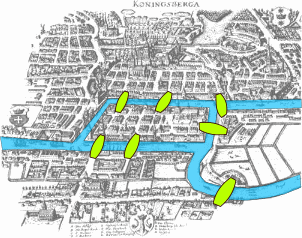
\includegraphics[width=\textwidth]{fig/bridges_map}
\end{minipage}
\begin{minipage}{0.45\linewidth}
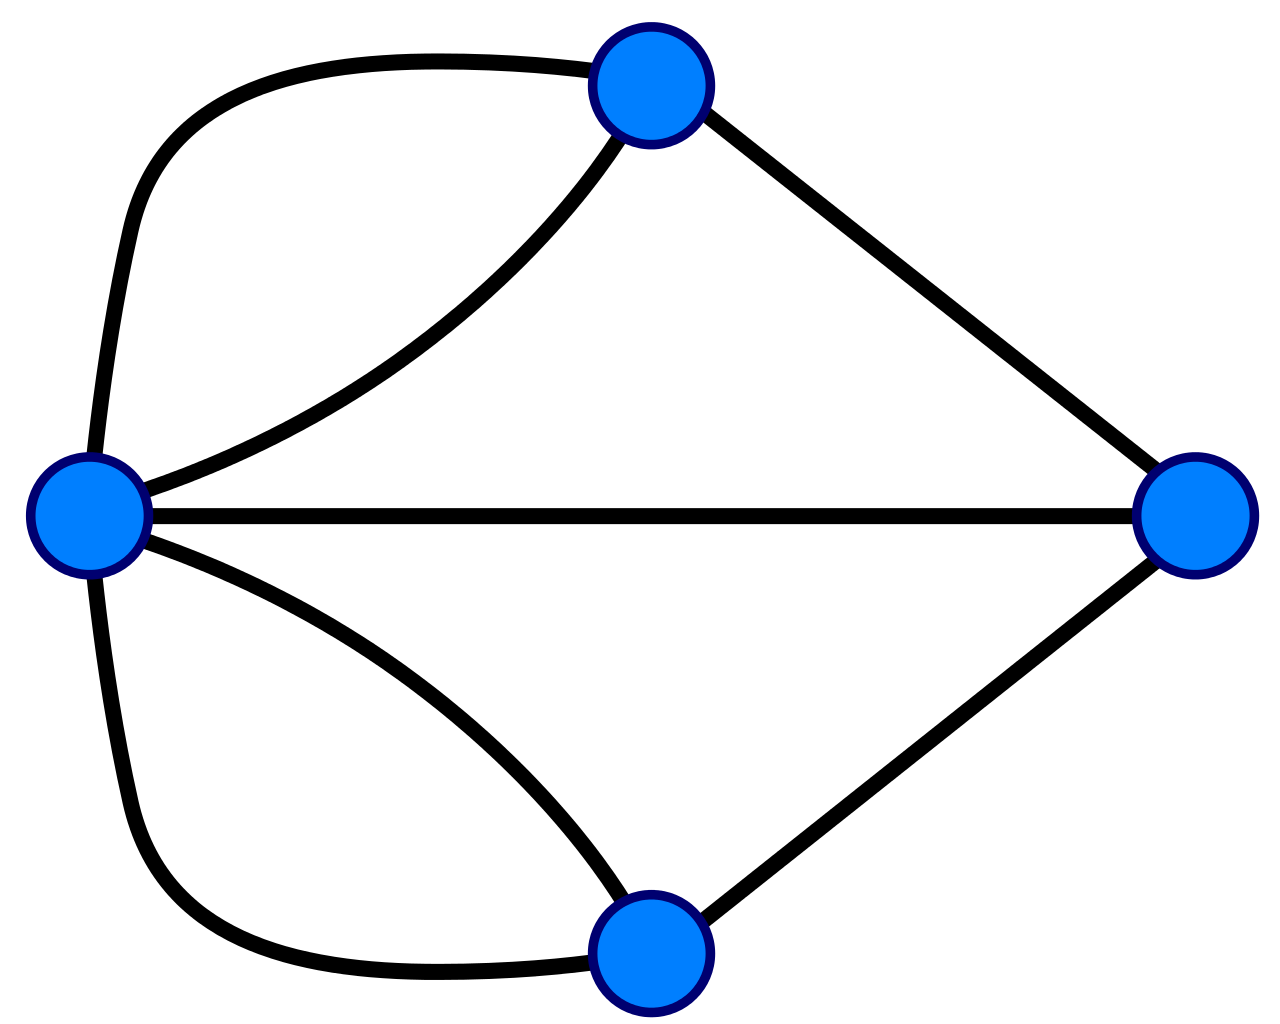
\includegraphics[width=\textwidth]{fig/bridges_graph}
\end{minipage}
\caption{The bridges of K\"onigsberg, as a map and a multigraph}
\label{fig:bridges}
\end{figure}

The bridges of K\"onigsberg spawned the traveling salesman problem (TSP) and what is seen as the first proof in the field of network science~\cite{newman2003structure}. The graph (shown in \autoref{fig:bridges}) is an illustrative example of the 

\subsection{K\textsubscript{3,2}}

\subsection{Florentine families}


   \chapter{INSULARITY AS A MEASURE OF NETWORK ROLES} \label{ch:insularity}% Must have a blank line after every section label

\section{Introdution} \label{sec:insularity introduction} % Must have a blank line after every section label

Insularity is computed from the LP in a manner similar to Mann's computation of flowthrough centrality; however, it is a dynamic property of the network: a function of the network's utilization. 

Flowthrough centrality is computed by solving the HMCFP to the point of total saturation; it is related to the node's the node's capacity (its weighted degree, a property of the graph) and the amount of flow terminating at that point, which is given in the solution of the HMCFP. 

\section{Results}

Stuff

   \chapter{RESULTS} \label{ch:results}% Must have a blank line after every section label
        %  2. Chapter 2
   
   \chapter{CONCLUSION} \label{ch:conclusion}% Must have a blank line after every section label

Summary of the problem, the main findings and the discussion. Structured according to the issues in Related Literature and Theoretical Focus.

Comparison with the literature: how do your results fill in, advance or contradict previously reported research?

What are the implications of your research for people working in the field that you have studied?

In which direction should further research go?

\section{Overview of Significant Research Results} \label{sec:Overview} % Must have a blank line after every section label

\section{Comparison to Popular Methods}

\section{Sensitivity and Robustness}

\section{The Insularity Measure}

\section{Future Work}



%-----------------------------------------------------------
%   Appendices go here if no appendix, remove \StartAppendix
%-----------------------------------------------------------
   \StartAppendix           %  All chapters from this point are treated as appendices
   
   \chapter{RELEVANT BACKGROUND IN LINEAR PROGRAMMING} \label{app:LP}% Must have a blank line after every section label

This appendix presents an operational description of linear programming (LP), a method of constrained optimization for linear systems of inequalities. Linear programs are the common method for solving the maximum concurrent flow problem (MCFP) and hierarchical MCFP (HMCFP). For greater detail, the reader is directed to Luenberger and Ye~\cite{luenberger2008linear} or Chvatal~\cite{chvatal1983linear}.

\section{Linear Programming}

Linear programming optimizes an objective function that is constrained by linear equalities and inequalities. For some linear objective function $z = c \transpose x$, we want to find the $x$ that maximizes $z$ while constrained by a system of linear inequalities $Ax \leq b$. 

A linear program in standard form comprises three parts:
\begin{enumerate}
\item A linear \say{cost} function to be maximized, e.g. $ z(x_{1},x_{2}) = c_1 x_1 + c_2 x_2$
\item Problem constraints, e.g.
\begin{equation}
\begin{matrix}
  a_{11} x_1 + a_{12} x_2 &\leq b_1 \\
  a_{21} x_1 + a_{22} x_2 &\leq b_2 \\
  a_{31} x_1 + a_{32} x_2 &\leq b_3 \\
\end{matrix}\end{equation}
\item Non-negative variables, e.g.
\begin{equation}\begin{matrix}
 x_1 \geq 0 \\
 x_2 \geq 0
\end{matrix}\end{equation}
\end{enumerate}
Problems with equality constraints or bounds other than non-negativity can be converted into these three parts; the reader is directed toLuenberger~and Ye~\cite{luenberger2008linear}. The problem is usually expressed in matrix form, and then becomes:
\begin{equation}
\max \{ %
\mathbf{c} \transpose
\mathbf{x} \;|\;
 \mathbf{A} \mathbf{x} \leq \mathbf{b} \land \mathbf{x} \geq 0 \}
\end{equation}

These linear constraints form half-planes that bound a convex polytope (a bounded polyhedron)~\cite{nemhauser1988integer}. Any point inside this polytope is a \emph{feasible solution}. 

Solving a linear program (when a solution exists) gives an optimal basis~$\mathbf{B}$. This basis is a matrix of  For a given basis, there is a corresponding \emph{basic solution}~$(\mathbf{x_B}, \mathbf{0})$. Here, $\mathbf{0}$ is the zero vector. The solution only has values for each $x_i$ corresponding to a column in $\mathbf{B}$. At most, $m$ of its entries are nonzero, where $m$ is the number of columns in A. (Here, we assume as for our problem that the number of rows $n \geq m$. 

\section{Shadow Prices and Sensitivity}

Every linear program has a corresponding dual program in the form:

\begin{equation}
\min \{ %
\bm{\lambda} \transpose
\mathbf{b} \;|\;
\bm{\lambda} \transpose \mathbf{A} \geq \mathbf{c} \transpose \land \bm{\lambda} \geq 0 \}
\end{equation}

The solutions to the dual program provide \emph{shadow prices}~$\bm \lambda$. The shadow prices reflect the marginal utility of relaxing the corresponding constraint in the primal, or the marginal cost of tightening the constraint:

\begin{align}
\lambda_i = \frac{\partial z}{\partial b_i}, \quad \forall i \in \{1, 2, \ldots, |\lambda|\}
\end{align}

These shadow prices are piecewise linear, and the particular range over which some shadow price~$\lambda_i$ is valid can be computed~\cite{luenberger2008linear}: when a value in $\mathbf{b}$ is altered, the values of the right-hand side in the optimal tableau are altered. The stable range is the interval along which the right-hand side of the tableau remains nonnegative. 

\section{Practical Considerations}

LPs can be quickly solved using the simplex method~\cite{puterman2014markov}. Although the method scales exponentially with input size in the worst case, average-case performance is far better. Additional methods have been proposed with polynomial worst-case behavior, such as interior point methods.
          %  Appendix A

%-----------------------------------------------------------
%   Bibliography goes below
%   Check with specific department on the appropriate
%   bibliography style to use
%-----------------------------------------------------------
   \nocite{*}
   \bibliographystyle{acm}
   \raggedright
%   \footnotesize           % For smaller font on Bibliography
   \bibliography{thesisbib}
%   \normalsize             % Uncomment to return to normal font after smaller font

%-----------------------------------------------------------
%   END body of the thesis
%-----------------------------------------------------------
  \end{thesis}

%===========================================================
%   END thesis document
%===========================================================

\end{document}
%===========================================================
% END Document
%===========================================================
